\documentclass[tikz,border=8pt]{standalone}
\usetikzlibrary{arrows.meta,positioning,fit,decorations.pathreplacing}
\begin{document}
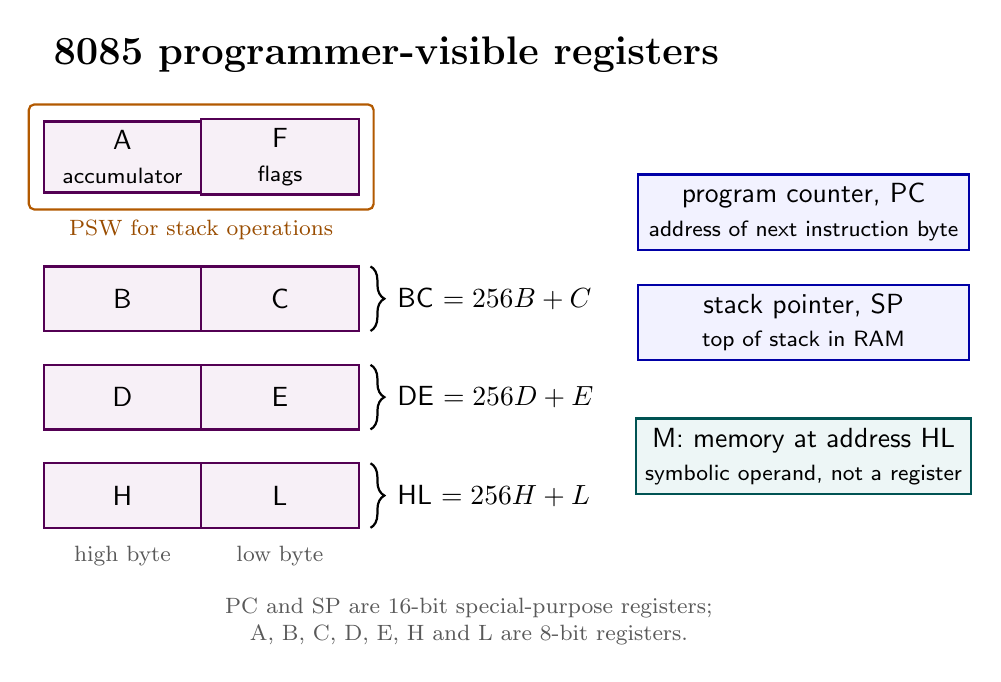
\begin{tikzpicture}[
  font=\sffamily,
  byte/.style={draw=violet!65!black,thick,minimum width=2.0cm,minimum height=.82cm,align=center,fill=violet!6},
  special/.style={draw=blue!65!black,thick,minimum width=4.2cm,minimum height=.9cm,align=center,fill=blue!5}
]
  \node[font=\bfseries\Large] at (4.45,3.35) {8085 programmer-visible registers};

  \node[byte] (a) at (1.1,2.05) {A\\\footnotesize accumulator};
  \node[byte] (f) at (3.1,2.05) {F\\\footnotesize flags};
  \node[draw=orange!70!black,rounded corners=2pt,thick,fit=(a)(f),inner sep=5pt,label={[font=\footnotesize,text=orange!60!black]below:PSW for stack operations}] {};

  \node[byte] (b) at (1.1,.25) {B};
  \node[byte] (c) at (3.1,.25) {C};
  \node[byte] (d) at (1.1,-1.0) {D};
  \node[byte] (e) at (3.1,-1.0) {E};
  \node[byte] (h) at (1.1,-2.25) {H};
  \node[byte] (l) at (3.1,-2.25) {L};

  \draw[decorate,decoration={brace,amplitude=5pt},thick] (4.25,.66) -- node[right=6pt]{BC $=256B+C$} (4.25,-.16);
  \draw[decorate,decoration={brace,amplitude=5pt},thick] (4.25,-.59) -- node[right=6pt]{DE $=256D+E$} (4.25,-1.41);
  \draw[decorate,decoration={brace,amplitude=5pt},thick] (4.25,-1.84) -- node[right=6pt]{HL $=256H+L$} (4.25,-2.66);
  \node[font=\footnotesize,text=black!65] at (1.1,-3.02) {high byte};
  \node[font=\footnotesize,text=black!65] at (3.1,-3.02) {low byte};

  \node[special] (pc) at (9.75,1.35) {program counter, PC\\\footnotesize address of next instruction byte};
  \node[special] (sp) at (9.75,-.05) {stack pointer, SP\\\footnotesize top of stack in RAM};
  \node[special,draw=teal!65!black,fill=teal!7] (m) at (9.75,-1.75) {M: memory at address HL\\\footnotesize symbolic operand, not a register};

  \node[font=\footnotesize,align=center,text=black!65] at (5.5,-3.85) {PC and SP are 16-bit special-purpose registers;\\A, B, C, D, E, H and L are 8-bit registers.};
\end{tikzpicture}
\end{document}
